\chapter{JIAC Node Plugin}
\label{sec:user_jiac-node}

Not actually a part of the VSDT, but closely related, is the so-called \emph{JIAC
Node Plugin}, which will be the topic of this chapter.

The central part of the JIAC Node Plugin is -- as the name suggests -- a JIAC
agent node~\cite{lutzenberger2013jiacShort} running \emph{inside} of an Eclipse
plug-in, which can be used as a platform for several applications, integrating
features provided by JIAC agents (both running on the node itself \emph{and} on
other nodes in the network) with into the Eclipse environment.

In the following, we will introduce two especially graphic applications for the
JIAC Node Plugin: The \emph{Multicast-Chat} and the \emph{Service-Deployment
View}.  Both of those views can be found in the \emph{DAI-Labor} group in the
views menu.


%%%%%%%%%%%%%%%%%%%%%%%%%%%%%%%%%%%%%%%%%%%%%%%%%%%%%%%%%%%%%%%%%%%%%%%%%%%%%%%%
%%  JIAC Multicast-Chat View                                                  %%
%%%%%%%%%%%%%%%%%%%%%%%%%%%%%%%%%%%%%%%%%%%%%%%%%%%%%%%%%%%%%%%%%%%%%%%%%%%%%%%%

\section{JIAC Multicast-Chat View}

The \emph{JIAC Multicast-Chat} was the first application developed for the JIAC
Node Plugin.  It is, in essence, a simple Chat application running inside of
Eclipse, making use of JIAC communication infrastructure.  While not being overly
useful, given the abundance of existing chat programs, the ease of integrating a
chat view into Eclipse using the JIAC Node Plugin is compelling.  Therefore, the
Multicast-Chat can also be seen as an elaborate tutorial for developing other
JIAC-based Eclipse plug-ins.

\begin{figure}[ht]
	\centering
	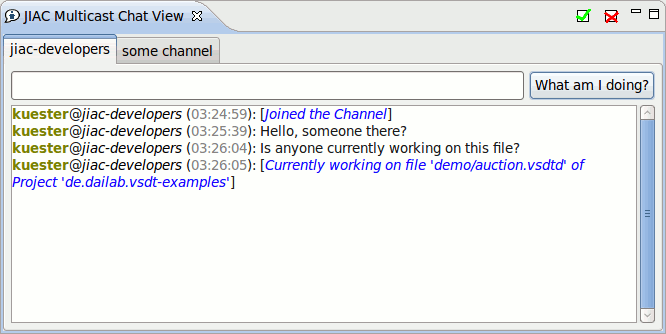
\includegraphics[width=.5\textwidth]{figures/features/multicast-chat.png}
	\caption{The JIAC Multicast-Chat View.}
	\label{fig:chatView}
\end{figure}

The Multicast-Chat View, as seen in Figure~\ref{fig:chatView}, allows the user to
subscribe to one or more chat channels, each one corresponding to a multicast
group channel in JIAC.  The user can then send messages to fellow developers being
subscribed to the same channel.  Since the multicast-chat is aimed especially at
developers working in their Eclipse IDEs at the same time, a special feature of
the Multicast-Chat is to broadcast which file of code one is currently working
on, possibly alleviating problems due to conflicting changes on that file.


%%%%%%%%%%%%%%%%%%%%%%%%%%%%%%%%%%%%%%%%%%%%%%%%%%%%%%%%%%%%%%%%%%%%%%%%%%%%%%%%
%%  JIAC Service-Deployment View                                              %%
%%%%%%%%%%%%%%%%%%%%%%%%%%%%%%%%%%%%%%%%%%%%%%%%%%%%%%%%%%%%%%%%%%%%%%%%%%%%%%%%

\section{JIAC Service Deployment View}

Another, much more useful view is the \emph{JIAC Service Deployment View}, shown
in Figure~\ref{fig:deployView}.  This view uses JIAC's service-discovery and
-invocation mechanisms to provide a number of features to the user:

\begin{itemize}
	\item \emph{Look up} services currently being provided by other JIAC agents in
	the network, displaying them in a tree view, grouped by agent and agent node,

	\item \emph{import} those services (both actions provided by JIAC agent beans
	and JADL services) as Service descriptions into the current VSDT diagram, so
	they can be reused and orchestrated to new services,

	\item \emph{deploy} new services composed in the VSDT\footnote{VSDT Process
	Diagrams will be exported to JADL services prior to being deployed on the
	JADL interpreter.} or in the JADL editor to some JADL interpreter agent
	currently running on some node,

	\item \emph{invoke} services and actions being provided by some JIAC agent on
	the network, including the ones just deployed, and

	\item \emph{undeploy} services.
\end{itemize}

\begin{figure}[ht]
	\centering
	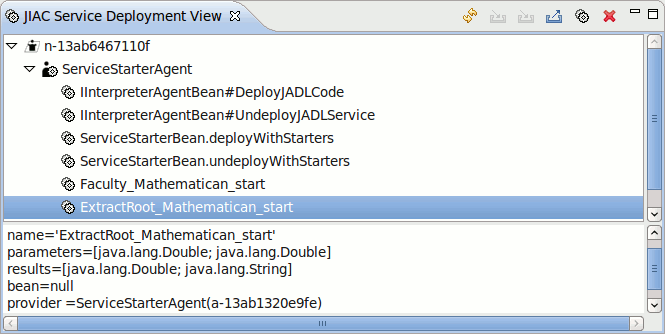
\includegraphics[width=.5\textwidth]{figures/features/deployment-view.png}
	\caption{The JIAC Service Deployment View.}
	\label{fig:deployView}
\end{figure}

While there are still some restrictions, e.g. service invocation from the
Deployment View currently works only for services with basic input and output
types (numbers, strings, etc.), these features are extremely helpful for developing
or composing new JIAC services -- both using the VSDT or the basic JADL source
code editor.

